%%%%%%%%%%%%%%%%%%%%%%%%%%%%%%%%%%%%%%%%%%%%%%%%%%%%%%%%%%%%%%%%%%%%%%%%%%%%%%%%
%2345678901234567890123456789012345678901234567890123456789012345678901234567890
%        1         2         3         4         5         6         7         8

\documentclass[letterpaper, 10 pt, conference]{ieeeconf}  % Comment this line out if you need a4paper


%\documentclass[a4paper, 10pt, conference]{ieeeconf}      % Use this line for a4 paper

\IEEEoverridecommandlockouts                              % This command is only needed if 
                                                          % you want to use the \thanks command

\overrideIEEEmargins                                      % Needed to meet printer requirements.

%In case you encounter the following error:
%Error 1010 The PDF file may be corrupt (unable to open PDF file) OR
%Error 1000 An error occurred while parsing a contents stream. Unable to analyze the PDF file.
%This is a known problem with pdfLaTeX conversion filter. The file cannot be opened with acrobat reader
%Please use one of the alternatives below to circumvent this error by uncommenting one or the other
%\pdfobjcompresslevel=0
%\pdfminorversion=4

% See the \addtolength command later in the file to balance the column lengths
% on the last page of the document


\usepackage{mathptmx} % assumes new font selection scheme installed
%\usepackage{times} % assumes new font selection scheme installed
\usepackage{amsmath}
\usepackage{amssymb}
\usepackage{multicol}
\usepackage[bookmarks=true]{hyperref}
\usepackage{mathptmx}
\usepackage[T1]{fontenc}
\usepackage{authblk}
\usepackage{graphicx}
\usepackage{relsize}		% For \smaller
\usepackage[linesnumbered]{algorithm2e}
\usepackage{subcaption}
\usepackage{makecell}
\usepackage{pgfplots}
\usepackage{multirow}
\usepackage{booktabs,caption}
\usepackage[flushleft]{threeparttable}
\usepackage{epsfig}

%commands
\DeclareRobustCommand{\rchi}{{\mathpalette\irchi\relax}}
\newcommand{\irchi}[2]{\raisebox{\depth}{$#1\chi$}} %

\newcommand{\marc}[1]{\textbf{\texttt{\color[rgb]{0,0,.8}#1}}}

\DeclareMathOperator*{\maxB}{max}
\DeclareMathOperator*{\argmaxB}{argmax} 
\DeclareMathOperator*{\minB}{min}
\DeclareMathOperator*{\argminB}{argmin}

\usetikzlibrary{positioning,fit,calc}
\tikzset{
block/.style={
draw,
thick,
text width=1.1cm,minimum height=1.5cm,align=center},
line/.style={-latex},
font={\fontsize{8pt}{12}\selectfont}
}

%title
\title{\LARGE \bf
Combined Task and Motion Planning under Partial Observability: An Optimization-Based Approach
}


\author{\textbf{Camille Phiquepal \space\space\space\space\space\space\space\space\space\space\space\space Marc Toussaint}\\
Machine Learning \& Robotic Lab, University of Stuttgart\\
\{firstname.surname\}@ipvs.uni-stuttgart.de
       }


\begin{document}



\maketitle
\thispagestyle{empty}
\pagestyle{empty}


%%%%%%%%%%%%%%%%%%%%%%%%%%%%%%%%%%%%%%%%%%%%%%%%%%%%%%%%%%%%%%%%%%%%%%%%%%%%%%%%
\begin{abstract}

  We propose a novel approach to Combined Task and Motion Planning
  (TAMP) under partial observability. Previous optimization-based TAMP
  methods [1][2] compute optimal plans and paths for a deterministic
  setting. However, partial observability requires the solution to be
  a policy that reacts to the observations that the agent receives. We
  consider a formulation where observations introduce additional
  branching in the symbolic decision tree. The solution is now given
  by a reactive policy on the symbolic level together with a
  \emph{path tree} that describes the branchings of optimal motion
  depending on the observations. Our method works in two stages:
  First, the symbolic policy is optimized using approximate path costs
  estimated from independent optimizations of trajectory pieces.
%Under this assumption, the decision process is markovian and policies are optimized using Value Iteration and Rmax algorithm.
Second, we fix the best symbolic policy and optimize a joint trajectory tree.
We test our approach on object manipulation and autonomous driving examples. We also compare the algorithm's performance to a state-of-the-art TAMP planner in the fully observable case.
\end{abstract}


%%%%%%%%%%%%%%%%%%%%%%%%%%%%%%%%%%%%%%%%%%%%%%%%%%%%%%%%%%%%%%%%%%%%%%%%%%%%%%%%
\section{Introduction}

Robots must combine the ability to reason symbolically about discrete actions (task planning) and geometrically about the realization in the real world (motion planning). Integrated approaches are referred to in the literature as  Task and Motion Planning (TAMP). 
With the exception of [4], current TAMP research assumes full observability. However partial observability is pervasive in many real world situations, e.g.\ when objects are hidden or partially hidden. If some objects to manipulate
are inside containers, the robot has to explore its environment to perform its task. Self driving cars face the same problem when operating in the presence of other vehicles that limit the field of view of the ego vehicle.

In this paper we extend the Logic-Geometric Programming  (LGP) approach [1,2]  to handle partial observability. Under partial observability, policies need to be reactive due to observations. In this paper, rather than focussing on control noise as in stochastic optimal control, we focus on  observations at discrete points in time that reveal essential information for the task. E.g., whether an object is in a container or not, or whether a car is approaching in the opposite lane. In this case, not only the symbolic policy needs to be reactive, also the optimal motion needs to branch at observations. Computing an optimal motion plan now means to compute an optimal trajectory tree. Our TAMP solver works in two stages: First piece-wise optimization and then joint tree optimization. During the first stage, the trajectories of actions are optimized independently (piece-wise).
%
%
In the second stage, we fix the best symbolic policy obtained in the first stage and optimize the joint trajectory tree that corresponds to this symbolic policy. I.e., instead of optimizing the sequential motion of each action in isolation, the whole trajectory tree is optimized all at once.

\section{Related Work}

Concerning Combined Task and Motion Planning, a number of approaches [5][8][9] rely on the discretization of the configuration spaces or action/skeleton parameters to leverage CSP methods. Prior work [1][2] states TAMP problems as an optimization problem. These approaches assume full observability and plan a single sequence of actions together with a single path. To our knowledge, the system in [4] is the only other TAMP planner considering partial observability. A \textit{Look} action is used to actively move the robot sensor to acquire information. This approach (Hierarchical Planning in the Now) interweaves planning with execution (in the now).
%Sequences of actions are planned by approximating the system dynamics (results of actions and observations).
Replanning is triggered once the robot ends up in a state not covered by the plan. In contrast, our approach aims at planning a full reactive policy from the starting state to the final state. In addition, we aim for smooth and locally optimal trajectories.

%Planning for autonomous driving also entails a layered decision making process with a combination of symbolic decisions and planning in a continuous space. [6][7] provide a surveys about planning for self-driving cars. To our knowledge, there exists no literature on TAMP approaches for decision making in the automotive context. 

\section{Problem Formulation}

\subsection{Overview}

We formulate the problem in terms of a decision tree and, for every action edge in this tree, cost and constraint objectives on the continuous trajectory. The decision tree is in belief space, including action and observation branchings. To define a problem we first define the symbolic partially observable decision process that spans this tree. Second, we define the cost and constraints functions that define the optimization objectives for the continuous trajectory problem associated with transitioning through this tree. An optimal policy is then comprised of a reactive policy that transitions the tree depending on observations, and an optimal trajectory tree which, depending on observations, smoothly switches into different motion options. To our knowledge, this is the first approach to propose trajectory trees as optimal reactive motion plans in the case of partial observability.

\subsection{Decision Process}

We assume a decision process defined by a 7-tuple $(S, A, T, \Omega, O, \gamma, G)$, where
\begin{itemize}
\item $S$ is a finite set of states
\item $A$ is a finite set of actions
\item $T$ is a set of conditional transition probabilities between states
\item $\Omega$ is a finite set of observations
\item $O$ is a set of conditional observation probabilities
\item $\gamma$ is a discount factor
\item $G$ is a set of goal conditions defined over the belief state space. A goal condition indicates if a decision tree node is terminal or not.
\end{itemize}
This is a POMDP except for the missing reward structure, which we replace by the associated trajectory optimization problems defined below. In addition, we have a goal condition over the belief space.

Given the initial belief $b_0$, the decision process spans a decision tree with two kinds of nodes:
\begin{itemize}
\item In \emph{action nodes} the agent has to choose which action to take; action nodes have $|A|$ children.
\item In \emph{observation nodes} the agent receives an observation; observation nodes have $|\Omega|$ children.
\end{itemize}
Every node in the tree corresponds a belief state computed with the standard belief update.

\subsubsection{Example for a decision graph}

Consider a car behind a truck. The car wishes to overtake but cannot see the opposite lane because of the truck, see Fig.~\ref{fig:overtaking}. The car can take three actions: look into the opposite lane, overtake the truck, or continue to follow the truck. After looking into the lane (move slowly toward the center of the road), the car receives an observation (lane free or not). Fig.~\ref{fig:overtaking-decision-graph} is the decision graph of this problem, assuming loop detection to turn the tree into a graph. The blue node is the start belief state. The green nodes are terminal belief states.
\marc{why is there not all three actions (look, overtake, stay) possible in the blue state??}
\marc{why does the (follow truck) go back to the blue initial state? We now know that the lane is free? Or because it might become non-free? And why is the left (follow truck) thing different?}

\begin{figure}\centering
  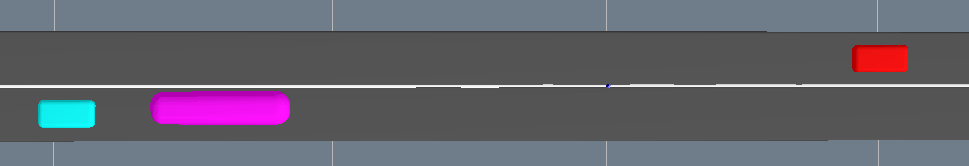
\includegraphics[width=0.5\textwidth]{images/overtaking.png}
  \caption{\label{fig:overtaking} The ego vehicle
    (cyan) wants to overtake but cannot observe if a vehicle arrives
    in the opposite direction because of the truck.}
\end{figure}
    
\begin{figure}\centering
  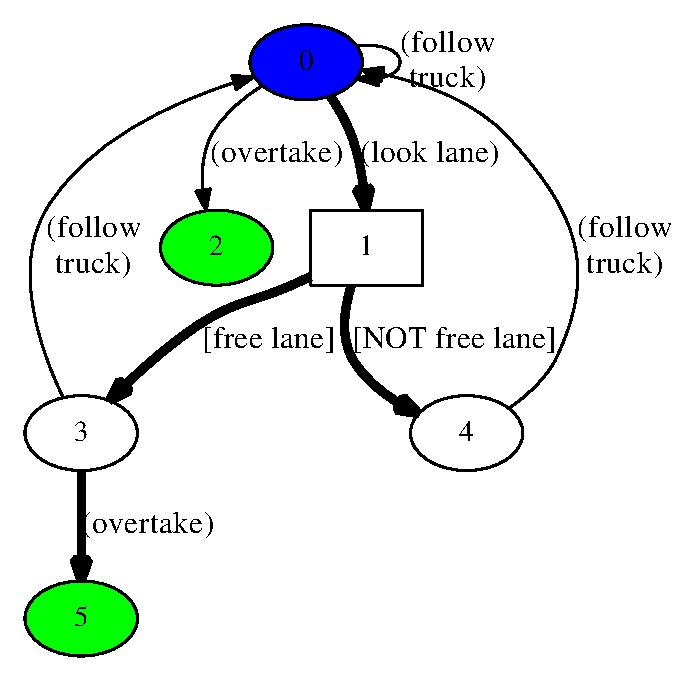
\includegraphics[height=0.25\textwidth]{images/graph.eps}
  \caption{\label{fig:overtaking-decision-graph} Decision graph for overtaking, the thick edges represent a possible policy}
\end{figure}

\subsubsection{Policy}

A policy $\pi$ is a mapping from belief states to actions. The thick edges in Fig.~\ref{fig:overtaking-decision-graph} represent a possible policy. The decision graph potentially contains cycles, however, in the following, we will only consider policies that are trees. In the case of full observability, the policy would boil down to a single sequence of actions. A policy reaching the goal condition, on the symbolic level, is a tree whose leafs are terminal belief states. We call this a candidate policy.

The observation model $O$, the initial belief state at the root node $b_0$, and the policy $\pi$ define the prior probability of reaching any given node $b$ in the decision tree. We will denote this probability by $p(b | \pi, b_0)$.

\subsection{Trajectory Trees}

The decision process described above defines sets of candidate policies that, on the symbolic level, reach goal conditions. As there are no rewards defined, all candidate policies are equal. However, on the geometric level, some candidate policies may be infeasible or lead to different path costs. We define here the path optimization problem associated with a candidate policy.

In typical trajectory optimization, the optimization objective is given as a set of constraints and sum of cost terms along the trajectory. In our setting, we generalize this to a set of constraints and sum of cost terms for each action edge in the tree, weighted by the probability of being in the corresponding belief.

More formally, let $\rchi$ be the configuration space of the whole environment, including the robot and all object configurations. Consider that
the agent takes an action $a \in A$ at a belief node $b$. We assume this implies cost and constraint functions on the trajectory during the time interval $[t_k, t_{k+1}]$. Namely, let $x$ be a trajectory in $\rchi$ over $[t_k, t_{k+1}]$, taking action $a$ implies costs
\begin{align}\label{eqCost}
c(a, x) = \int_{t_k}^{t_{k+1}} & {f_a(x(t), \dot{x}(t), \ddot{x(t)}) ~dt}\\
\text{if}~~  & g_a(x(t), \dot{x}(t), \ddot{x(t)}) \le 0\\
& h_a(x(t), \dot{x}(t), \ddot{x(t)}) = 0 ~.
\end{align}
and $c(a,x) = +\infty$ if the constraints are not satisfied by path $x$.

Planning motions in the partially observable case means that we need to have motions pre-computed for all cases, i.e., for all observations that might happen during execution. This means that our planner computes trajectory pieces $x$ for all action edges in the decision tree. Together, they form a trajectory tree. We require this tree to be smooth at its ramifications (which is implicit in smoothness costs and equality constraints). We use $\psi$ to denote a full trajectory tree.

\subsection{Optimal Policy and Trajectory Tree}

We can now define the problem as finding a symbolic policy $\pi$ and a trajectory tree $\psi$ that minimize the expected cost,
\begin{equation}
\Pi^* = \argminB_{(\pi, \psi)} \sum_{b\in\pi} p(b | \pi, b_0)~ \gamma^{k(b)}~ c(\pi(b), \psi(b)) ~,
\end{equation}
given the initial belief $b_0$. Here, the expectation is w.r.t.\ the probability of visiting a belief node in the decision tree, and discounted with gamma.

\section{Solver}

We propose a solver that works in three stages, schematized on Fig.~\ref{fig:algo}. First, the decision graph is build. Second, we alternate Value Iteration and piece-wise trajectory optimization to compute the symbolic policy $\pi^*$ jointly with a set of trajectory pieces. These pieces do not yet form a globally optimal trajectory tree, but inform the symbolic policy optimization about the cost and feasibility associated with actions. In the third stage we fix $\pi^*$ and optimize the full trajectory tree jointly.

The optimization of trajectory pieces in stage 2 raises substantial computational costs. Therefore our solver involves several mechanisms to decide on whether it is worth to ``explore'' actually computing these trajectory pieces. These mechanisms include using a simple approximation to check feasibility, and a mechanism akin to Rmax [3] to decide on whether an action should be ``explored''.

\begin{figure}
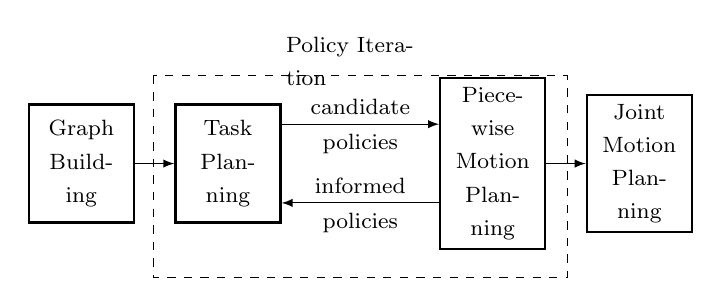
\begin{tikzpicture}
  \node[block] (a) {Graph Building};
  \node[block, right=0.5cm of a] (b) {Task Planning};
  \node[block, right=2cm of b] (c) {Piece-wise Motion Planning};
  \node[block, right=0.5cm of c] (d) {Joint Motion Planning};
  %\coordinate [left=of c] (b_output);
  \draw[line] (a)-- (b);
  \draw[line] ([yshift=0.5cm] b.east)-- ([yshift=0.5cm] c.west) node[pos=0.5,above]{candidate} node[pos=0.5,below]{policies};
  \draw[line] ([yshift=-0.5cm] c.west)-- ([yshift=-0.5cm] b.east) node[pos=0.5,above]{informed} node[pos=0.5,below]{policies};
  \draw[line] (c)-- (d);
%  \node (rect) [rectangle, draw, minimum width=70mm, minimum height=100mm, anchor= south west] at (0,0) {};
  \draw [draw=black,dashed] ([xshift=-0.95cm, yshift=0.35cm] b.north) rectangle ([xshift=0.95cm, yshift=-0.35cm,label=$m$] c.south);
%  \draw [decorate,decoration={brace,amplitude=10pt},xshift=0pt,yshift=0pt]
%([xshift=-0.55cm] b.north) -- ([xshift=0.55cm] c.north);
\node[text width=2cm] at (3.6,1.3) {Policy Iteration};
\end{tikzpicture}
\caption{TAMP algorithm}
\label{fig:algo}
\end{figure}

\subsection{Graph Building} 

The decision graph, is expanded from the start belief state using a breadth first strategy. In the general case, the number of reachable belief states is infinite, leading to an infinite decision graph. We limit the graph size by expanding only to a certain maximal depth.

\subsection{Value Iteration on the decision graph} \label{ssec:dp}

We assume that at any point in time we have cost estimates $c(a,b)$ for each action $a$ in belief state $b$. However, these costs are all initialized with a low, optimistic number, as in Rmax. Only when an optimal policy makes it likely to actually visit $(a,b)$ we compute more precise estimates using piece-wise trajectory optimization, as described below.

Given $c(a,b)$ we use Value Iteration
\begin{equation}
V^{\star}_{i+1}(b) \leftarrow \min_{a} \big[ c(a, b) + \gamma \sum_{o \in O(b, a) } O( o | b, a ) V^{\star}_{i}(T(b, a, o))
\big]
\end{equation} 
until convergence to compute the value function for all belief nodes. Non-terminal (non-goal) leaf nodes are initialized with infinite value; terminal leaf nodes with zero value. This defines the optimal policy $\pi^*$ w.r.t.\ the current estimates $c(a,b)$.

\subsection{Piece-wise Trajectory Optimization} \label{ssec:top}

A given policy $\pi^*$ transitions only a small subset of action edges of the full decision graph. For this set of action edges we compute $c(a,b)$ (if it was not already computed in previous iterations). For the sake of computational efficiency, we estimate $c(a,b)$ in two stages:

We first optimize key-frames only (robot pose at each node). This step is much quicker than optimizing a full trajectory piece. If an action is impossible during the feasibility check, the optimization is not pursued further. In addition, this node and its sub-tree are labeled infeasible (with infinite costs) and thereby unreachable by the optimal policies. The pose feasibility check is optimistic, it might succeed even if the path itself is infeasible (no possible trajectory without collision between two key-frames for example).

If pose optimization reports feasibility, we then optimize the trajectory piece $x$, minimizing (\ref{eqCost}), to get the cost estimate $c(a,b)$. We use a time discretization of 20 frames per action. In addition to the cost and constraint functions defined by the action, the robot dynamics and collision avoidance are included. The trajectory optimization methods are adopted from [1][2]. We save the cost $c(a,b)$, the computed trajectory piece $x$, and in particular its final configuration for this action edge.

There may be a strong overlap between candidate policies generated by Value Iteration (same edge in many candidate policies). This is especially the case in the last iterations of Policy improvement, saving computational costs as computing $c(a,b)$ is performed only once. Intuitively, as we alternate between Value Iteration and evaluating relevant trajectory pieces, the decision graph is filled with geometric information.

 
\subsection{Initialization of $c(a,b)$ and graph exploration}\label{ssec:explo}

The use of optimistic initializations of $c(a,b)$ is analogous to the Rmax algorithm [3] and allows us to control exploration vs.\ exploitation within the policy optimization. An optimistic initial $c(a,b)$ (e.g., zero costs) encourages exploration. This Rmax mechanisms in combination with Value Iteration can be viewed as an alternative to other exploration mechanisms in tree search, such as admissible heuristics, or UCB in the probabilistic case. In our particular use case, we do not have uncertainty about the transitions, but only about the costs (negative rewards) as we were lazy to compute them. This relates well to the notion of ``unknown states'' in Rmax model-based reinforcement learning.

On the other hand, when initializing $c(a,b)$ less optimistic, we loose the guarantees that come with admissible heuristics, but may converge faster to reasonable policies. Our experiments will investigate the influence of the cost initialization on the number of iterations.
 
\subsection{Joint Optimization of the Trajectory Tree}

In the third stage of the solver, we fix the symbolic policy $\pi^*$ found as described so far, and focus on the joint optimization of the trajectory tree $\psi$. So far we have only computed pieces $x$ for each action edge. Concatenating these independently optimized pieces cannot capture long-term dependencies in the trajectories, e.g.\ when final actions influence earlier parts of the trajectory. The autonomous driving example will exemplify this, when the velocity early in the trajectory tree should depend on the probability that an overtake maneuver will be possible. The joint optimization of the trajectory tree leads to better and smoother motions. It is computationally costly, but performed only once for the best symbolic policy $\pi^*$.

We again solve the problem stage-wise. We first optimize all linear trajectories from the root to each one of the reached terminal belief nodes \emph{independently} (see $opt\_1$ and $opt\_2$ on Fig.~\ref{fig:joint}). Secondly, the trajectories are re-optimized with additional equality constraints enforcing that the common parts between trajectories are identical (see $opt\_3$ and $opt\_4$). The re-optimization is potentially performed multiple times until the equality constraints across trajectories are fully satisfied (in practice, one iteration is often enough).
%\marc{weighed $\to$ weighted in the figure}

This procedure is akin to ADMM (Alternating Direction Multiplier Method), where we decomposed the tree problem into multiple linear trajectory problems, but introduce additional equality constraints to tie the common parts. Each linear trajectory problem can be addressed using efficient path optimization methods, exploiting its Markovian structure (e.g., banded-diagonal Hessian) [1][2]. ADMM is guaranteed to converge to the joint optimum and recently received great attention as a means to decompose and parallelize large structured optimization problems.

\begin{figure}[h!]
  \centering
      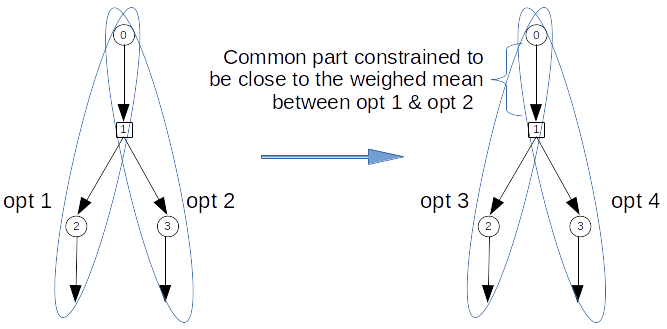
\includegraphics[height=0.2\textwidth]{images/tree-joint_2.png}
  \caption{Joint optimization}
  \label{fig:joint}
\end{figure}

\section{\label{sec:experiments} Experimental Results}

\subsection{Block stacking with the Baxter}
We consider a Baxter robot wiht three blocks on a table (see Fig.~\ref{fig:block-world}). The robot has to stack the blocks in a given color order (blue, green, and red on the top). The blocks just have one side colored (assumed to be the opposite side). The robot knows where the blocks are (referred as $block\_1$, $block\_2$, $block\_3$). However it cannot see the colored side from behind and has explore to identify the blocks and to build the stack in the correct order. Only the robot right arm is assumed to be able to grasp.
\begin{figure}
\centering
        \begin{subfigure}[t]{0.18\textwidth}
            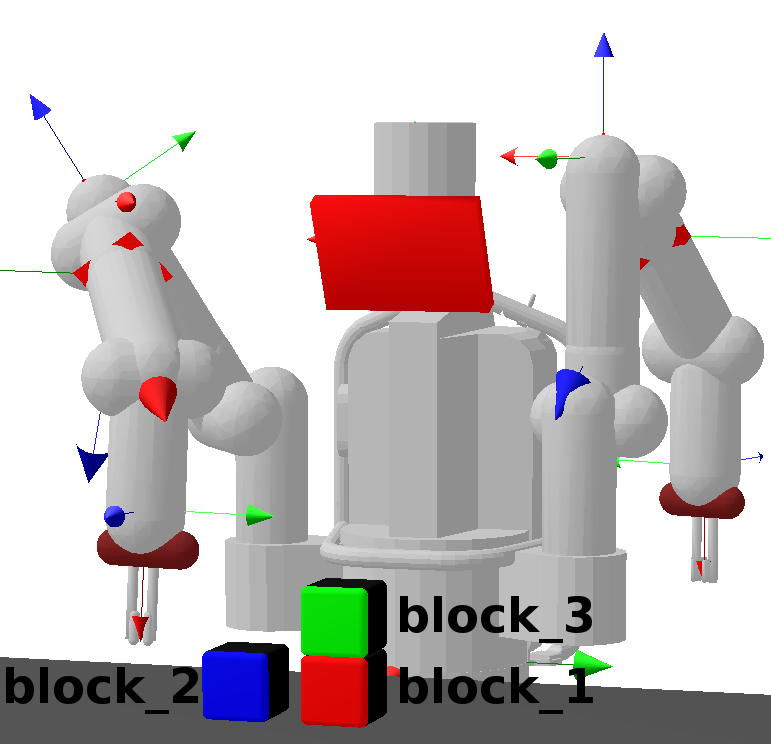
\includegraphics[width=\textwidth]{images/start-a.png}
            \caption{\label{fig:start-1}first start configuration with model B}
        \end{subfigure}
        \hfill
        \begin{subfigure}[t]{0.18\textwidth}
            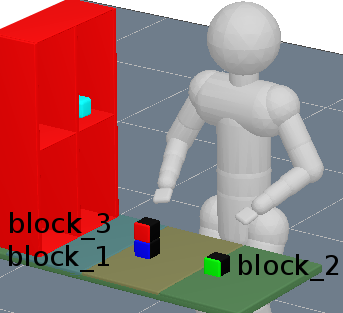
\includegraphics[width=\textwidth]{images/start-b.png}
            \caption{\label{fig:start-2}second start configuration with model B}
        \end{subfigure}
        %\hfill
        \hfill
        \begin{subfigure}[t]{0.18\textwidth}
            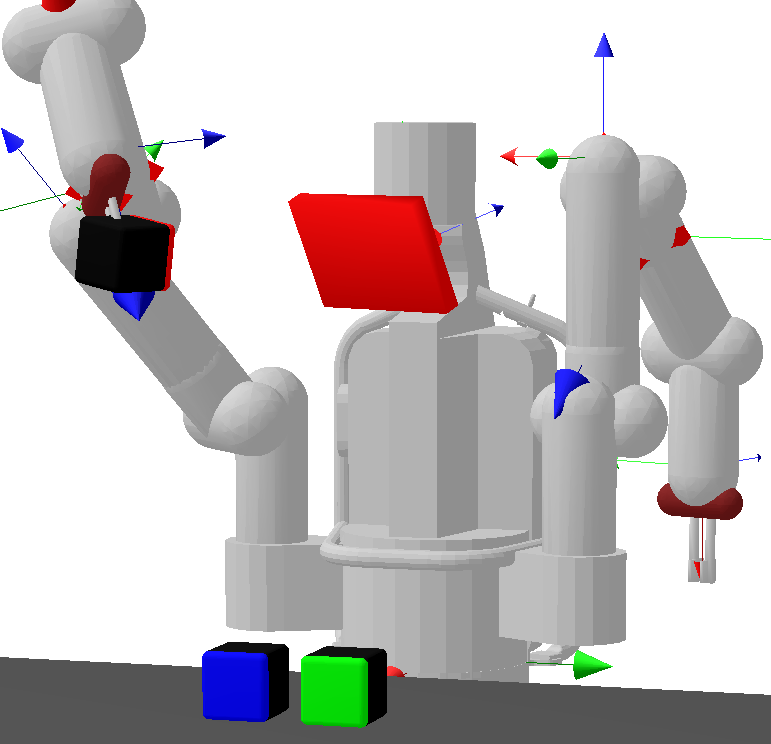
\includegraphics[width=\textwidth]{images/look.png}
            \caption{\label{fig:look-1}\textit{Look} with the block in hand}
        \end{subfigure}
        \hfill
        \begin{subfigure}[t]{0.18\textwidth}
            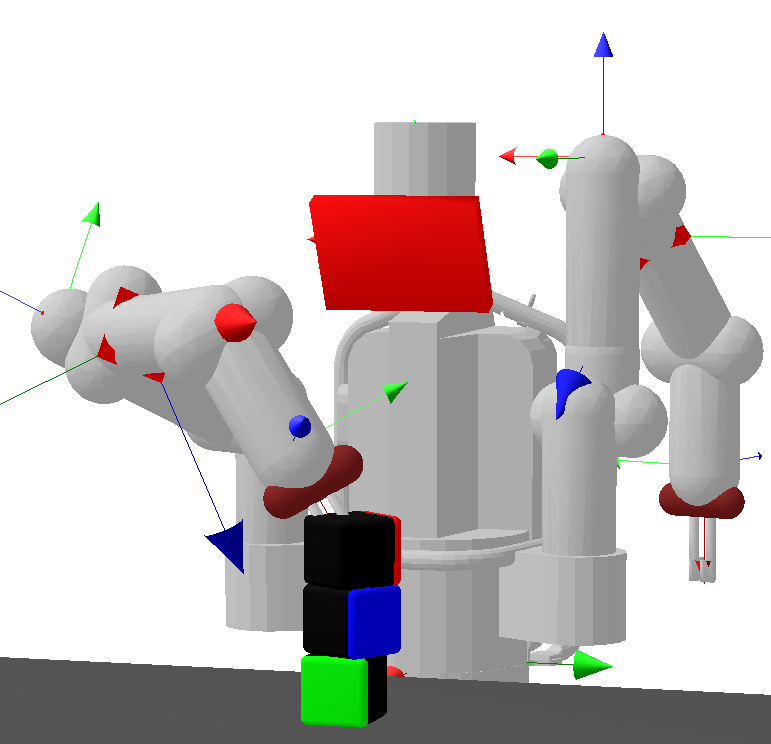
\includegraphics[width=\textwidth]{images/goal.png}
            \caption{example of goal configuration}
        \end{subfigure}
        \caption{\label{fig:block-world}Example of configurations. The robot must stack the blocks in a given color order. The block colors are not visible from behind}
\end{figure}
There are 3 possible actions: 
\begin{itemize}
\item \textbf{Look} at a block: the robot seeks to align its sensor (assumed to be the robot head) with the colored side of the box. This will typically lead the robot to both move its head and its arm simultaneously (see Fig.~\ref{fig:look-1}). After this action, the robot receives an observation (color of the block).
\item \textbf{Grasp} a block: only the right arm can grasp
\item \textbf{Place} a block at a location: the block is placed on the table location, or onto another block.
\end{itemize}

%We evaluate two different action models. In the first variation (Variation 1), the action \textit{Look} has a symbolic precondition: the robot should be holding a block before checking it. This precondition is not present in the second variation (Variation 2). The \textit{Look} action is possible more often which increases the branching factor and the size of the decision graph. However, most of the time, when the robot doesn't hold a block, the \textit{Look} action is infeasible geometrically: Indeed the robot has to place place its head far ahead and look backwards which is, in most cases, infeasible given the geometrical constraints of the robot. It is however interesting to note, that this is possible in some cases (if the robot has just previously placed the block close to the table border with some orientation see Fig.~\ref{fig:look-2}). In other words, the grasp-precondition is not absolutely necessary to ensure the feasibility of the \textit{Look} action. This variation is used to analyze how our approach works with a more ``free'' albeit not invalid symbolic problem description causing a lot of motion planning failures.%

%\begin{figure}
%\centering
%        \hfill
%        \begin{subfigure}[t]{0.15\textwidth}
%            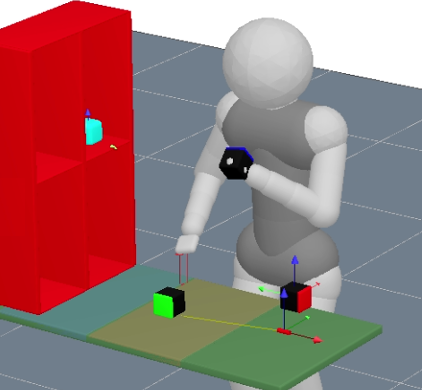
\includegraphics[width=\textwidth]{images/suss-b.png}
%            \caption{\label{fig:look-1}\textit{Look} with the block in hand}
%        \end{subfigure}
%        \hfill
%        \begin{subfigure}[t]{0.15\textwidth}
%            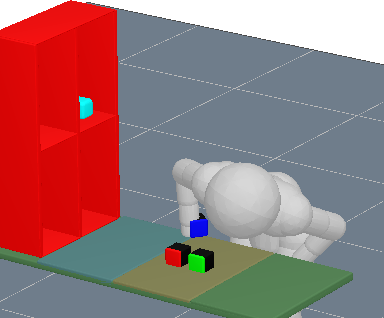
\includegraphics[width=\textwidth]{images/check-no-lift.png}
%            \caption{\label{fig:look-2}\textit{Look} just after having posed a block}
%        \end{subfigure}
%        \hfill
%        \caption{\label{fig:checks}Example of geometric configurations reached after the \textit{Look} action}
%\end{figure}

To evaluate the scalability, we test with three different initial belief states configurations. In the first configuration (A), the agent has a prior knowledge of the color of each block. This boils down to the fully observable case, no \textit{Look} action is needed. In the second configuration (B), 2 blocks are unknown. Fig.~\ref{fig:start-1} and ~\ref{fig:start-2} show the two possible start configurations with this model. In the third case (C), there are no prior knowledge which leads to 6 possible initial configurations. In all cases, the initial belief state is uniform (e.g. 1/2 likelihood for each possible start configuration with the model B, 1/6 likelihood for model C).

To evaluate the robustness against motion planning failure, we evaluate two different action models. In the first variation (Variation 1), the action \textit{Look} has a precondition: the robot should be grasping a block before checking it. This precondition is not present in the second variation (Variation 2). This introduces a lot of motion planning failures. Indeed, in most cases, no head movement allows the robot to align with the colored side of the block if the block is not grasped.
The different start configurations are summed up in the table \ref{table:problems}.
\begin{center}
\footnotesize
\setlength\tabcolsep{3pt} % default value: 6pt
\begin{tabular}[ht]{|c|c|c|c||c|c|c|}
\hline
\thead{} & \thead{Belief state\\ size} & \thead{Blocks\\known} & \thead{Grasp\\ \textit{precondition}} & \thead{Graph\\size} & \thead{Graph\\building time(s)} \\
\hline
A                     & 1 & \thead{3/3} &\thead{-} &  63 & 0.023 \\
\hline
B1                    & 2 & \thead{1/3} &\thead{yes} & 196 & 0.083 \\
\hline
B2                    & 2 & \thead{1/3} &\thead{no} &  234 & 0.11 \\
\hline
C1                    & 6 & \thead{0/3} &\thead{yes} & 1084 & 0.69 \\
\hline
C2                    & 6 & \thead{0/3} & \thead{no} & 1486 & 1.18 \\
\hline
\end{tabular}
\captionof{table}{\label{table:problems}Summary of the considered problem variations} 
\end{center}

\begin{figure}[h!]
  \centering
  \hfill
  \begin{subfigure}[t]{0.31\textwidth}
      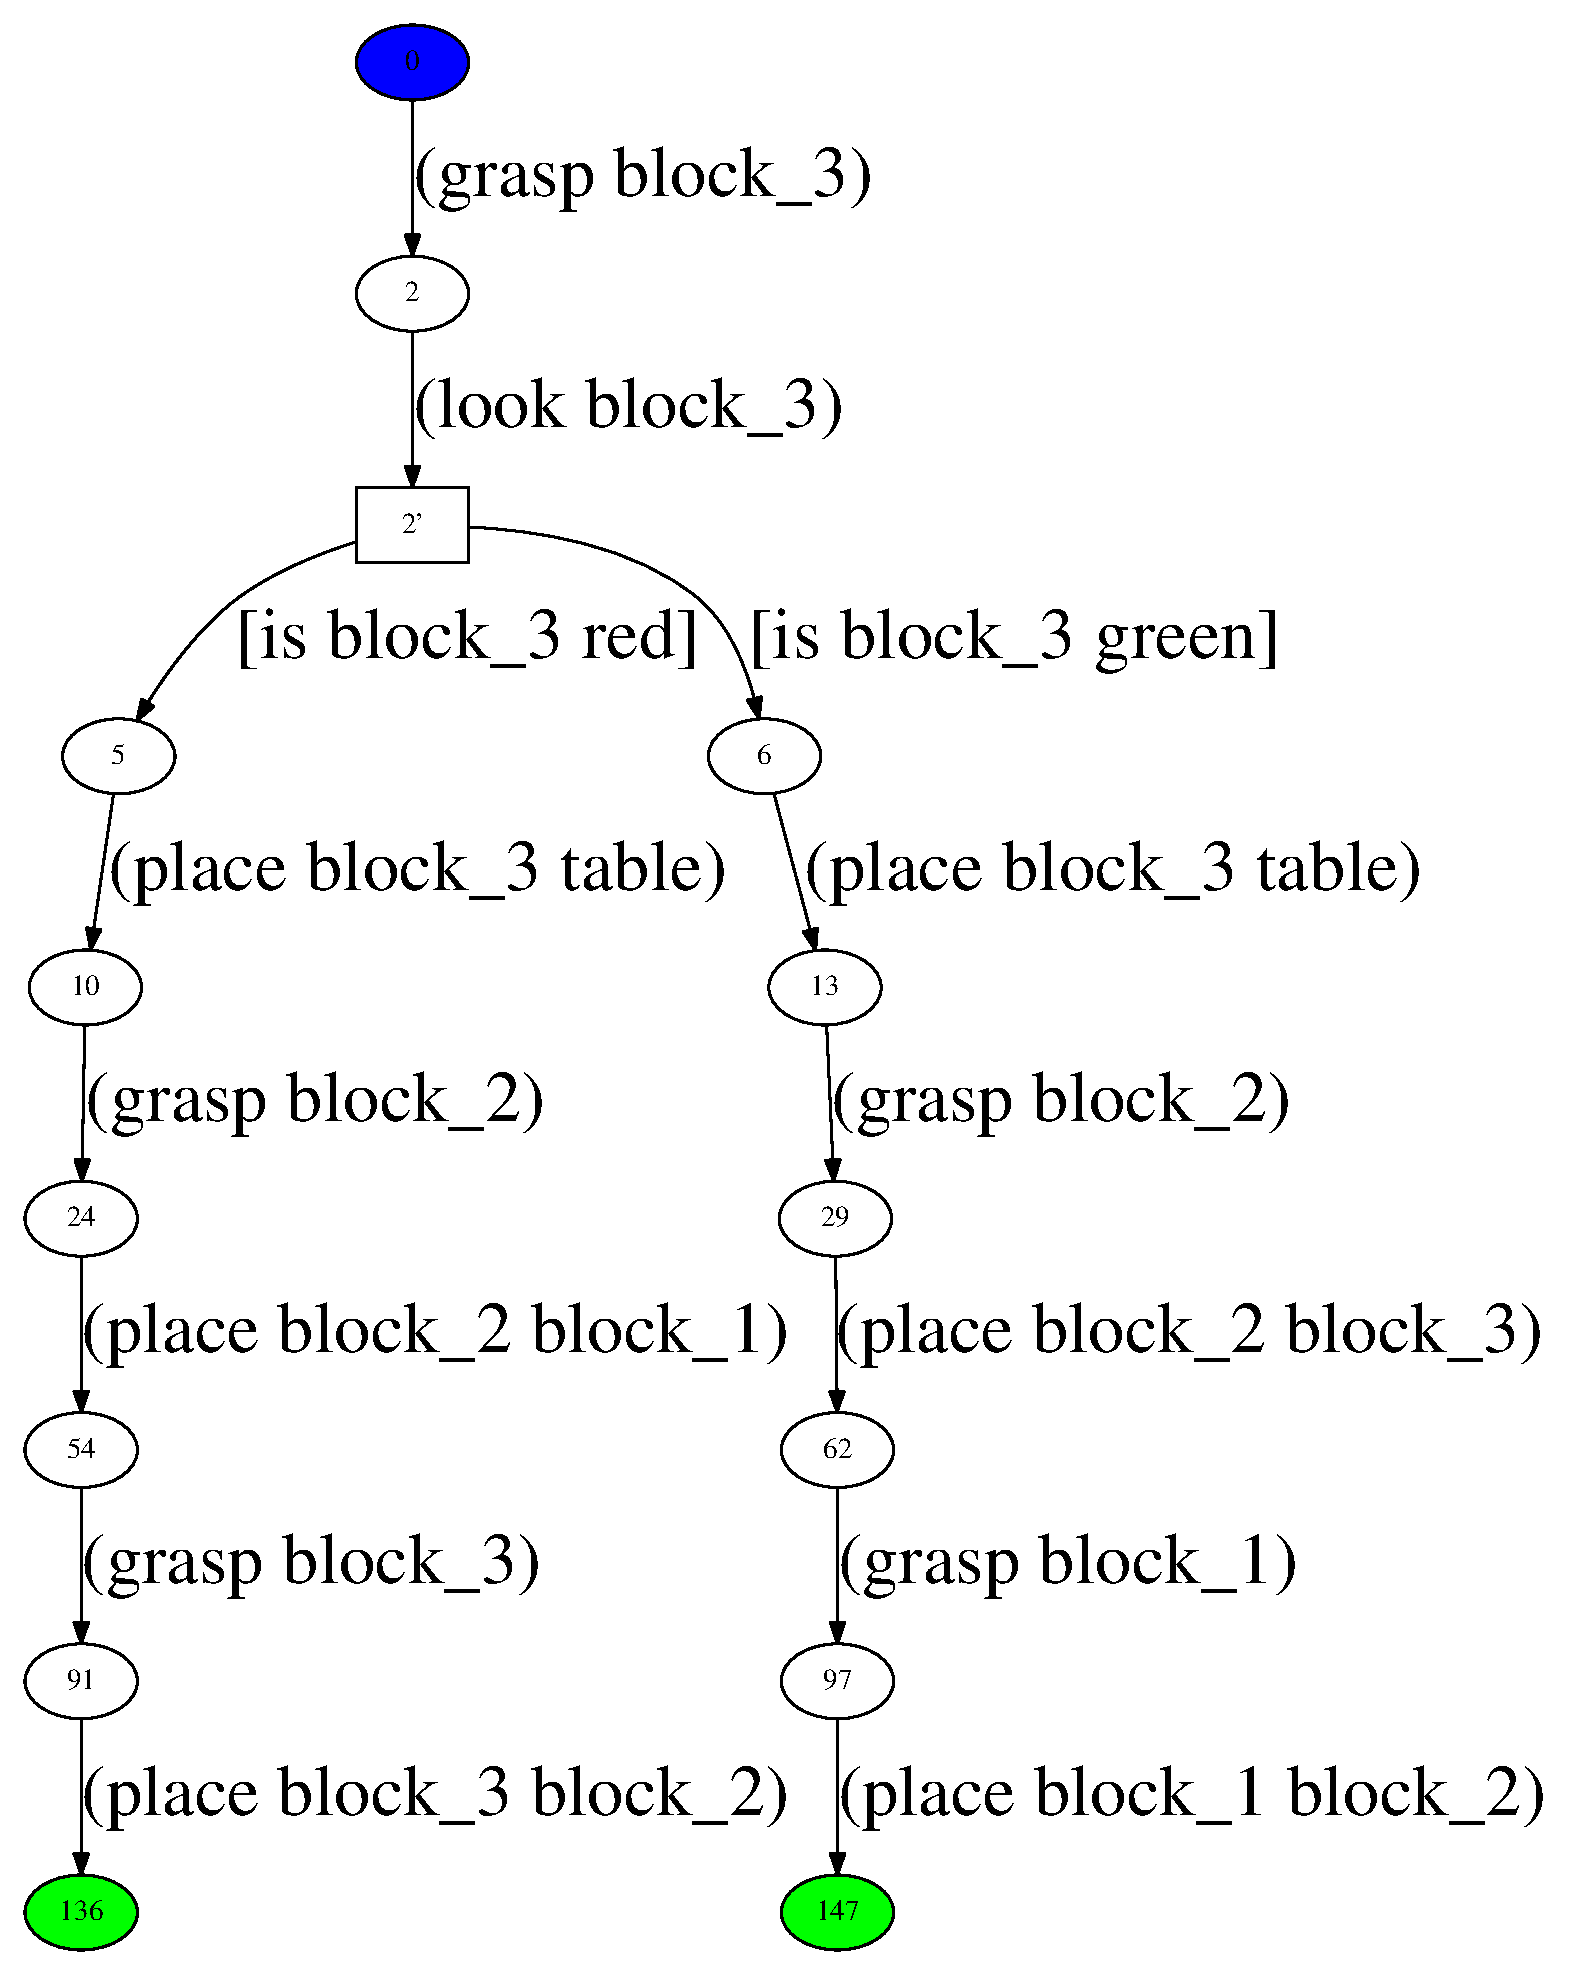
\includegraphics[width=\textwidth]{data/2m1/-0.015/10/policy-11-final-arranged.eps}
  \caption{\label{fig:policy-B2}result policy for B2. The block 3 is checked, then the stacking is continued sequentially}
  \end{subfigure}
  \hfill
  \begin{subfigure}[t]{0.15\textwidth}
      \includegraphics[width=\textwidth]{data/1m2/-0.25/10/policy-2-final.eps}
  \caption{\label{fig:policy-A2}result policy for A2}
  \end{subfigure}
\end{figure}

\begin{center}
\footnotesize
\setlength\tabcolsep{3pt} % default value: 6pt
\begin{tabular}{|c|c|c|c|c|c|c|c|}
\hline
                  			   & \thead{$C_0$} & \thead{Iter-\\ations} & \thead{N of\\actions*} & \thead{Task\\planning} & \thead{Piecewise\\motion\\planning} & \thead{Joint\\motion\\planning} & Total**\\
\hline
\multirow{3}{*}{A}     & 0.25  & 2 & 6 & 0.027 & 1.62 & 3.27 & 4.95 \\
				        & 0.1   & 2 & 6 & 0.034 & 1.67 & 3.54 & 5.27 \\
					    & 0.015 & 2 & 6 & 0.029 & 1.67 & 4.02 & 5.75 \\
\hline
\multirow{3}{*}{B1}     & 0.25  & 5 & 12 & 0.10 & 8.83 & 14.1 & 23.1 \\
				        & 0.1   & 5 & 12 & 0.10 & 8.02 & 15.1 & 23.3 \\
					    & 0.015 & 7 & 12 & 0.17 & 10.7 & 14.1 & 25.1 \\
					    
\hline
\multirow{3}{*}{B2}     & 0.25  & 20 & 12 & 0.45 & 8.64 & 23.2 & 32.4 \\
				        & 0.1   & 23 & 12 & 0.57 & 10.8 & 14.7 & 26.2 \\
					    & 0.015 & 30 & 12 & 0.75 & 28.2 & 14.3 & 43.4 \\
\hline
\multirow{3}{*}{C1}     & 0.25  & 11 & 33 & 0.81 & 42.6 & 66.9 & 111.0 \\
				        & 0.1   & 22 & 33 & 1.69 & 61.8 & 66.9 & 131.1 \\
					    & 0.015 & 41 & 37 & 2.07 & 321.3 & 112.7 & 444.1\\
\hline
\multirow{3}{*}{C2}     & 0.25  & 80 & 33 & 10.2 & 97.2 & 84.9 & 193.6 \\
				        & 0.1   & 199 & 33 & 27.6 & 234.2 & 86.2 & 349.2 \\
					    & 0.015 & 252 & 33 & 40.0 & 385.5 & 114.1 & 540.9 \\
\hline
\end{tabular}
\begin{tablenotes}
      \footnotesize
      \item * Number of actions of the final policy
      \item ** The total planning time also includes the graph building time given in the table \ref{table:problems}
    \end{tablenotes}
\captionof{table}{\label{table:times}Number of iterations and planning times} 

\end{center}

\begin{figure}[h!]
\begin{tikzpicture}
\begin{axis}[
    title={Values of candidate and result policies for B1},
    title style={yshift=-2ex},
    xlabel={Iterations},
    ylabel={Value},
    xmin=0, xmax=14,
    ymin=-2, ymax=0.6,
    xtick={0,1,5,10,15,20},
    ytick={-2,-1.5,-1,-0.5,0,0.5},
    legend pos=north west,
    legend columns=2, 
    legend style={font=\fontsize{7}{8}\selectfont},
    legend cell align={left},
    ymajorgrids=true,
    grid style=dashed,
    x label style={at={(axis description cs:0.5,0.05)},anchor=north}
]
   \addplot[ 
    color=purple,
    dashed,
    ]
    table [col sep=comma]{data/2m1/-0.25/10/policy-candidates.data};
    \addlegendentry{$candidate, C_0=0.25$}
    
\addplot[ 
    color=purple,
    ]
    table [col sep=comma]{data/2m1/-0.25/10/policy-results.data};
    \addlegendentry{$results, C_0=0.25$}
    
\addplot[ 
    color=blue,
    dashed,
    ]
    table [col sep=comma]{data/2m1/-0.1/10/policy-candidates.data};
    \addlegendentry{$candidate, C_0=0.1$}
    
\addplot[ 
    color=blue,
    ]
    table [col sep=comma]{data/2m1/-0.1/10/policy-results.data};
    \addlegendentry{$results, C_0=0.1$}    
 
\addplot[ 
    color=orange,
    dashed,
    ]
    table [col sep=comma]{data/2m1/-0.015/10/policy-candidates.data};
    \addlegendentry{$candidate, C_0=0.015$}
    
\addplot[ 
    color=orange,
    ]
    table [col sep=comma]{data/2m1/-0.015/10/policy-results.data};
    \addlegendentry{$result, C_0=0.015$}
             
\end{axis}
\end{tikzpicture}

%\begin{tikzpicture}
%\begin{axis}[
%    title={Values of candidate and result policies for B2},
%    title style={yshift=-2ex},
%    xlabel={Iterations},
%    ylabel={Value},
%    xmin=0, xmax=40,
%    ymin=-2, ymax=0.6,
%    xtick={0,5,10,15,20,25,30,35,40},
%    ytick={-2,-1.5,-1,-0.5,0,0.5},
%    legend pos=north west,
%    legend columns=2,
%    legend style={font=\fontsize{7}{8}\selectfont},
%    legend cell align={left},
%    ymajorgrids=true,
%    grid style=dashed,
%    x label style={at={(axis description cs:0.5,0.05)},anchor=north}
%]
%   \addplot[ 
%    color=purple,
%    dashed,
%    ]
%    table [col sep=comma]{data/2m2/-0.25/10/policy-candidates.data};
%    \addlegendentry{$candidate, C_0=0.25$}
    
%\addplot[ 
%    color=purple,
%    ]
%    table [col sep=comma]{data/2m2/-0.25/10/policy-results.data};
%    \addlegendentry{$result, C_0=0.25$}
           
%\addplot[ 
%    color=blue,
%    dashed,
%    ]
%    table [col sep=comma]{data/2m2/-0.1/10/policy-candidates.data};
%    \addlegendentry{$candidate, C_0=0.1$}
    
%\addplot[ 
%    color=blue,
%    ]
%    table [col sep=comma]{data/2m2/-0.1/10/policy-results.data};
%    \addlegendentry{$result, C_0=0.1$}
     
%\addplot[ 
%    color=orange,
%    dashed,
%    ]
%    table [col sep=comma]{data/2m2/-0.015/10/policy-candidates.data};
%    \addlegendentry{$candidate, C_0=0.015$}
    
%\addplot[ 
%    color=orange,
%    ]
%    table [col sep=comma]{data/2m2/-0.015/10/policy-results.data};
%    \addlegendentry{$result, C_0=0.015$}

%\end{axis}
%\end{tikzpicture}

\caption{\label{fig:convergences} Policy improvement over Value Iterations depending on the cost initialization $C_0$. The dashed line shows the cost estimates used by the algorithm, which use the prior cost $C_0$ for yet non-evaluated actions. The solid line shows the true costs, not known to the algorithm. (Red is a pessimistic initialization, where the true cost is lower than the prior cost $C_0=0.25$.)
}

\end{figure}


\subsubsection{Influence of $c(a,b)$ initialization}

\marc{Please only ever talk about costs, and lower is better. Please flip Fig. 7 to become a cost plot, not Value. It's confusing otherwise.}

Fig.~\ref{fig:convergences} displays the cost of policies over Value Iterations in two versions: the true costs (solid line), and the cost estimates that are used in the algorithm and use $C_0$ for actions that have not been optimized yet (dashed line). For strictly optimistic (admissible) $C_0$, the dashed line goes upward as more an more actions are evaluated.

With a pessimistic cost initialization of $C_0=0.25$, the search finishes as soon as a first policy is found. This happens after one single iteration with the B1. With the B2, the search encounters infeasible actions, the first possible policy is found at the 7th iteration. This policy is less optimal than the results found with the other initializations.

The lowest cost initialization of $C_0=0.015$ is always optimistic and leads to the most exploratory behavior. The cost of candidate policies (containing at least one unexplored action) are consequently always lower than the true cost. It requires the largest number of iterations. In particular, task planning also explores deeper policies (with more steps). In some cases a slightly deeper policy results in a better trajectory costs (see B2 with $C_0$ = 0.015). \marc{there is no plot for B2} The search converges to a better policy than with the other cost initializations. The small improvements in the last iterations are due to small rearrangements of the target location when placing blocks (e.g.\ place a block on table-left instead of table-center).

\subsubsection{Influence of the action precondition}

\marc{which plot should I look at??}

Removing the precondition increases strongly the decision graph size, and more iterations are needed.
%, and a majority of candidate policies are infeasible geometrically. This is visible on Fig.~\ref{fig:convergences} for the model B2 (below), the curves of result policies are very discontinuous because the majority of them are infeasible. Most of the time, Motion planning fails due to one single action. The trajectory costs of the actions that were sucessfully planned still inform the decision graph which enables the search to progress.
The search reaches an optimal policy which is as good as the policy obtained with the model with precondition. We think that this is an important quality of the proposed solution. Adding domain specific knowledge in the task planning (to ensure that motion planning will succeed) speeds up the search. However, in the general case, we think that it is not always possible / convenient to incorporate such geometric reasoning (reachability of a view point, reachability of an object) in the logical reasoning. 

\subsubsection{Execution time and scalability}

The overall planning time is dominated by the motion planning (see table.~\ref{table:times}). As long as the model is simple (A or B) or the exploration kept low ($C_0= 0.25$), motion planning is dominated by the single pass of joint optimization. The execution time of this pass mainly depends on the total number of action steps in the policy and on the belief state size but is independent from the number of iterations occurring before. In the configurations requiring the largest number of iterations (C1 and C2 with $C_0 = 0.015$), motion planning and the overall planning time are dominated by the piecewise motion planning phases of the policy improvement iterations. %It also appears clearly that scalability is a crucial problematic here. All the parameters of the problem increase drastically with the size of the belief state (graph size, required number of iterations, size of the resulting policy, computation time).%
Parameterizing the search with a very exploratory behavior may be feasible for problems of small sizes but suffers from the curse of dimensionality. One way to still enable some exploration while maintaining a bounded planning time is to save the best candidate policy planned so far and interrupt the iterations when a given time limit is reached.

\subsection{Comparison against another TAMP Planner}

We used the block example introduced above to benchmark the proposed solver against the \textit{Task Motion Kit} (TMKit) [10] in the fully-observable case. This solver implements the \textit{Incremental Task and Motion Planning} algorithm (IDTMP) (see [11]). We added a 4-th block in the example to further test the scalability. The benchmark was conducted on an Intel\textregistered Core\texttrademark i3-4100M CPU under Ubuntu 16.04. \ref{table:benchmark} shows planning metrics obtained by running each planner 100 times on each problem.
\begin{center}
\footnotesize
\begin{tabular}{|c|c|c||c|c|c|}
\hline 
\thead{} & \thead{Avg. path\\length} & \thead{std-dev} & \thead{Task\\Planning} & \thead{Motion\\Planning} & \thead{Total (s)}\\
\hline 
\thead{3 blocks\\LGP} & 4.03 & 0.04 & 0.10 & 2.88 & 2.98 \\		    
\hline 
\thead{3 blocks\\TMKit} & 3.28 & 1.08 & 1.84 & 6.09 & 6.98 \\	
\hline 
\thead{4 blocks\\LGP} & 5.79 & 0.04 & 0.36 & 4.62 & 4.98 \\		    
\hline 
\thead{4 blocks\\TMKit} & 7.54 & 1.12 & 11.32 & 20.39 & 31.72 \\		
\hline 
\end{tabular}
\captionof{table}{\label{table:benchmark}Planner comparison}
\end{center}
The proposed planner is faster than the TMKit for this given problem. We also report on path length but note that LGP actually optimizes for path smoothness (TMKit paths are not smooth). The trajectories planned with the LGP are similar across multiple runs (low standard deviation). On the other hand, the paths of the TMKit (obtained with the RRT-Connect algorithm) vary much more. 
One reason for the longer planning time of the TMKit lies in the interface between the Motion and Task Planner. Motion planning queries are composed of the start and goal pose of a given frame (robot end-effector or object). This requires to know the final pose before motion planning. To generate candidate goal poses, the surfaces where an object can be placed (e.g. the table) are discretized. This increases the branching factor of the search which makes it less efficient. Within the LGP framework, a motion planning problem is specified by a start pose plus cost and constraints functions. The final poses are naturaly obtained as a result of the trajectory optimization and don't rely on a discretization of the scene.

\subsection{Overtaking behavior}

We consider the overtaking problem introduced previously. Albeit simple, this example highlights the advantage of the joint (vs. piece-wise) trajectory-tree optimization which leads to anticipatory optimal trajectories. Fig.~\ref{fig:overtaking-decision-graph} is the decision graph and Fig.~\ref{fig:overtaking-start-configurations} shows two start configurations. In the first configuration $(a)$, the opposite lane is free enough to overtake. In $(b)$ overtaking is not possible. The Fig.~\ref{fig:overtaking-policy} shows the optimal policy. The trajectory cost of the action \textit{Look} is implemented as the distance between the car and the center of the road. It moves the car toward the center to get sight of the lane (see Fig.~\ref{fig:overtaking-look}). The action \textit{Follow} is implemented as a constraint which is satisfied if the ego-car is behind the truck (with a safety distance) at the end of the action. The action \textit{Overtake truck} is a constraint satisfied if the ego-car is in front of the truck.
\begin{figure}[h!]
  \centering
      \includegraphics[width=0.5\textwidth]{data/cars/policy.eps}
  \caption{Overtaking optimal policy}
  \label{fig:overtaking-policy}
\end{figure}

\begin{figure}[h!]
  \centering
  \begin{subfigure}[t]{0.5\textwidth}
      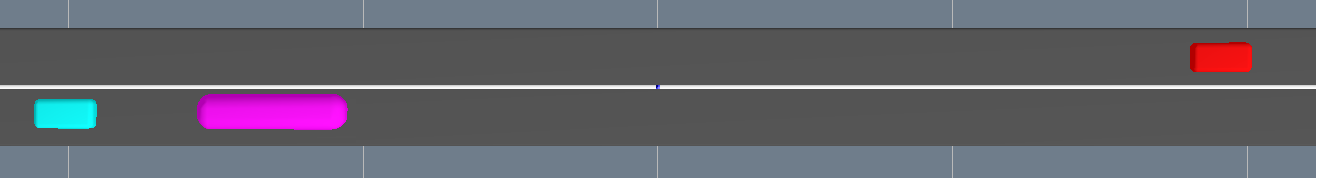
\includegraphics[width=\textwidth]{data/cars/start-0.png}
      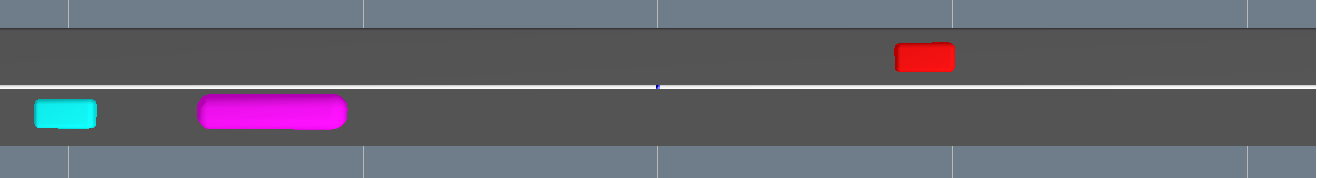
\includegraphics[width=\textwidth]{data/cars/start-1.png}
      \caption{\label{fig:overtaking-start-configurations}two start configurations}
  \end{subfigure}   
      
  \begin{subfigure}[t]{0.5\textwidth}
      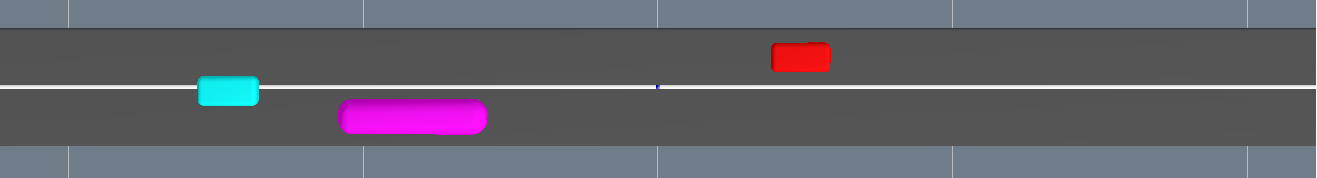
\includegraphics[width=\textwidth]{data/cars/look.png}
        \caption{\label{fig:overtaking-look}\textit{Look} action, the ego vehicle moved to the road center to observe the lanes}   
  \end{subfigure} 
  \begin{subfigure}[t]{0.5\textwidth}
      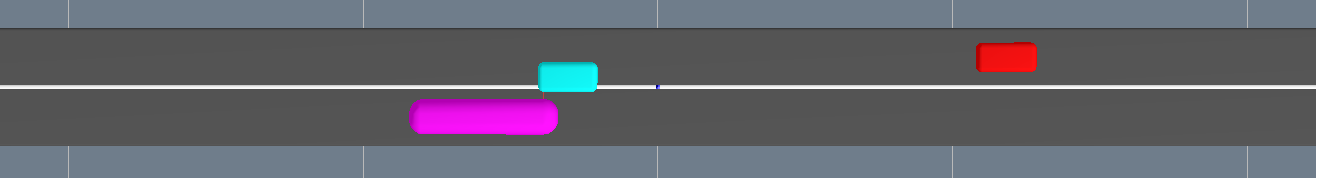
\includegraphics[width=\textwidth]{data/cars/overtaking.png}
        \caption{the ego vehicle overtakes (the opposite vehicle is far enough)}
  \end{subfigure}
  \begin{subfigure}[t]{0.5\textwidth}
      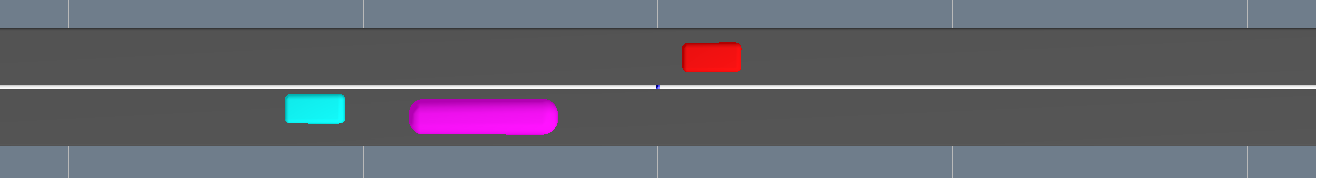
\includegraphics[width=\textwidth]{data/cars/follow.png}
      \caption{the ego vehicle moves back to its lane (opposite lane not free)}
  \end{subfigure}
\end{figure}

This example emphasizes the improvement brought by the joint trajectory optimization. The curves on Fig.~\ref{fig:overtaking-speeds} represent the longitudinal velocities of the trajectory tree for different planning configurations. At $t=6.5 s$, the car receives the observation $[lane\ free]$ or $[NOT\ lane\ free]$. If the lane is free, the car accelerates to overtake and then slows down once the truck is overtaken. Otherwise, the car slows down and move back to follow the truck.

\begin{figure}
\begin{tikzpicture}
\begin{axis}[
    %title={Vehicle Speed},
    xlabel={Time(s)},
    ylabel={Speed (m/s)},
    xmin=0, xmax=15,
    ymin=17.5, ymax=47.5,
    xtick={0,5,6.5,10,15},
    ytick={20, 30, 40, 45},
    legend pos=north west,
    legend columns=1,
    legend style={font=\fontsize{7}{8}\selectfont},
    legend cell align={left},
    ymajorgrids=true,
    grid style=dashed,
    x label style={at={(axis description cs:0.5,0.05)},anchor=north}
]
   \addplot[ 
    color=purple,
    style={very thick}
    ]
    table [col sep=comma]{data/cars/30-70/0.csv}node[above,pos=0.56] {$overtaking$};
    \addlegendentry{$ Joint\ Planning\ prior\ of\ p( lane\ free ) = 0.3$}
    
    \addplot[ 
    color=blue,
    style={very thick}
    ]
    table [col sep=comma]{data/cars/70-30/0.csv};
    \addlegendentry{$ Joint\ Planning\ prior\ of\ p( lane\ free ) = 0.7$}
    
    
    \addplot[ 
    color=gray,
    style={very thick}
    ]
    table [col sep=comma]{data/cars/fast/0.csv};
    \addlegendentry{$ Piecewise\ Motion\ Planning\ only$}
    
    \addplot[ 
    color=purple,
    style={very thick}
    ]
    table [col sep=comma]{data/cars/30-70/1.csv}node[below,pos=0.63] {$following\ truck$};
    %\addlegendentry{$joint 1$}
    
    \addplot[ 
    color=blue,
    style={very thick}
    ]
    table [col sep=comma]{data/cars/70-30/1.csv};
    %\addlegendentry{$ p( lane\ free ) = 0.7$}
    
    \addplot[ 
    color=gray,
    style={very thick}
    ]
    table [col sep=comma]{data/cars/fast/1.csv};
    
\end{axis}
\end{tikzpicture}
  \caption{\label{fig:overtaking-speeds}Longitudinal speed of the overtaking maneuver}
\end{figure}

The gray curve results from the piecewise motion planning. When looking at the lanes, the car keeps exactly the same speed (gray curve is flat for $t<6.5s$). When starting to overtake, the car is, still quite far from the truck and accelerates strongly to overtake. On the other hand, the blue and purple curves (Joint Optimization) are much smoother. To avoid a too strong acceleration, the car anticipates and accelerates slightly when looking. If overtaking is possible, the car pursues its acceleration, otherwise, it slows down and go back in the lane. We think that this mimics what human drivers do in case of ``tense'' overtaking maneuver. The initial belief state also influences the behavior. If it is likely that overtaking is possible ($0.7$ likelihood for the blue curve), the car will accelerate more when looking. In practice, the initial belief state could come from a service providing global information about the traffic in the area.

\section{Conclusion \& Future Work}

\marc{perhaps shorten}

We proposed a new, optimization-based approach to TAMP problems under partial observability.
It computes a reactive policy in the belief space, spanned by a symbolic decision graph, and a trajectory tree that allows the agent to reactively choose from pre-computed motion options depending on the observations. Thereby it can plan policies that combine exploratory actions (mostly sensor trajectories) and exploitative actions (e.g.\ grasp, place). Within planning, the degree of exploration over the space of all possible manipulations policies can be controlled by the cost initialization parameter, akin to Rmax.

Scalability becomes an issue when the number of manipulations and or the size of the belief state increases. An efficient way to speed-up the search is to have a task-level model that is accurately tailored for the problem to solve (example of the grasp precondition), this prevents too many motion planning failures and limits the branching factor. In future work, we intend to explore, how the task-level model can be refined and learned using the results from multiple planning queries.

Our current method computes policies that address every possible outcome of probabilistic observations. To scale better, we plan to investigate in an approach where the policy is planned only to handle the most probable belief state trajectories. As such a policy couldn't handle every outcome at execution time, re-planning would be triggered once the execution layer detects that the system is evolving toward a belief state which is not covered by the current policy.

%biblio
\begin{thebibliography}{99}

\bibitem{c1} M. Toussaint and M. Lopes, Multi-Bound Tree Search for Logic-Geometric Programming in Cooperative Manipulation Domains. Accepted at ICRA 2017.
\bibitem{c2} M. Toussaint, Logic-Geometric Programming: An Optimization-Based Approach to Combined Task and Motion Planning. In Proc. of the Int. Joint Conf. on Artificial Intelligence (IJCAI 2015), 2015.
\bibitem{c3} Brafman, Ronen I. and Tennenholtz, Moshe: {R-MAX} - a general polynomial time algorithm for near-optimal reinforcement learning. Journal of Machine Learning Research, Volume 3, 213-231, 2003
\bibitem{c4} Leslie Pack Kaelbling, Tomas Lozano-Perez. Integrated Task and Motion Planning in Belief Space, International Journal of Robotics Research, 2013
\bibitem{c5} T. Lozano-P�rez and L. P. Kaelbling. A constraint-based method for solving sequential manipulation planning problems. In Intelligent Robots and Systems (IROS 2014), 2014 IEEE/RSJ International Conference on, pages 3684-3691. IEEE, 2014
\bibitem{c6} Katrakazas, C., Quddus, M., Chen, W.-H., Deka, L.: Real-time motion planning methods for autonomous on-road driving: State-of-the-art and future research directions. Transp. Res. Part C 60, 416-442, 2015
\bibitem{c7} Paden, B., Cap, M., Yong, S.Z., Yershov, D., Frazzoli, E.: A survey of motion planning and control techniques for self-driving urban vehicles. IEEE Trans. Intell. Veh. 1(1), 33-55, 2016
\bibitem{c8} F. Lagriffoul, D. Dimitrov, A. Saffiotti, and L. Karlsson. Constraint propagation on interval bounds for dealing with geometric back-tracking. In Intelligent Robots and Systems (IROS), 2012 IEEE/RSJ International Conference on, pages 957-964. IEEE, 2012
\bibitem{c9} F. Lagriffoul, D. Dimitrov, J. Bidot, A. Saffiotti, and L. Karlsson. Efficiently combining task and motion planning using geometric constraints. The International Journal of Robotics Research, 2014
\bibitem{c10} N. T. Dantam, S. Chaudhuri, and L. E. Kavraki, Incremental Task and Motion Planning: The Task Motion Kit. IEEE Robotics and Automation Magazine, 2018
\bibitem{c11} N. T. Dantam, Z. K. Kingston, S. Chaudhuri, and L. E. Kavraki, Incremental Task and Motion Planning: A Constraint-Based Approach, in Robotics: Science and Systems, 2016


\end{thebibliography}
\end{document}

